\documentclass[aspectratio=169]{beamer}
\usefonttheme{serif}
\usepackage{xeCJK}
\usepackage{fontspec}
\usepackage{graphicx}
\usepackage{listings}
\usepackage{xcolor}
\usepackage{indentfirst}
\usepackage{tikz}
\usepackage{amssymb}
\usepackage{amsthm}
\usepackage{amsmath}
\usepackage{tabularx}
\usepackage{hyperref}
\usepackage{ulem}
\usepackage{version}
\usepackage{thmtools}
\usepackage{qtree}
\usepackage{algpseudocode}
\usepackage{mathtools}
\usepackage{multicol}
\usepackage{color}
\usepackage{ulem}
\usepackage{gensymb}
\usepackage{subfigure}


\AtBeginDocument{%
    \DeclareSymbolFont{pureletters}{T1}{lmr}{\mddefault}{it}%
}

\XeTeXlinebreaklocale "zh"
\XeTeXlinebreakskip = 0pt plus 1pt

\setCJKmainfont{NotoSansTC-Medium.otf}

\usetikzlibrary{arrows,decorations.markings,decorations.pathreplacing}
\newenvironment{Hint}{\noindent\textbf{Hint.}}{}

\tikzstyle {graph node} = [circle, draw, minimum width=1cm]
\tikzset{edge/.style = {decoration={markings,mark=at position 1 with %
            {\arrow[scale=2,>=stealth]{>}}},postaction={decorate}}}

\lstset{
    basicstyle=\ttfamily\tiny,
    % numberstyle=\small,
    % numbers=left,
    % stepnumber=1,
    % numbersep=3pt,
    commentstyle=\color{black!50},
    keywordstyle=\color{white!0!blue},
    stringstyle=\color{black!50!green},
    showspaces=false,
    showstringspaces=false,
    showtabs=false,
    tabsize=4,
    captionpos=b,
    breaklines=true,
    breakatwhitespace=false,
    escapeinside={\%*}{*)},
    morekeywords={*}
}
\AtBeginSection[]{
  \begin{frame}
  \vfill
  \centering
  \begin{beamercolorbox}[sep=8pt,center,shadow=true,rounded=true]{title}
    \usebeamerfont{title}\insertsectionhead\par%
  \end{beamercolorbox}
  \vfill
  \end{frame}
}

\title{計算幾何}
\author{sam571128}
\date{2022-07-15}

\usetheme{Madrid}
\usecolortheme{default}
\setbeamertemplate{itemize items}[square]
\setbeamertemplate{enumerate items}[default]
\setbeamertemplate{blocks}[default]

\begin{document}

\frame{\titlepage}

\begin{frame}{目錄}
    \begin{itemize}
        \item 先備知識
        \item 高中數學複習 - 向量
        \begin{enumerate}
            \item 什麼是向量
            \item 向量運算
            \item 正射影
        \end{enumerate}
        \item 用電腦存向量
        \item 浮點數誤差分析
        \item 向量的應用
        \item 凸包
        \item 旋轉卡尺
        \item 極角排序
        \item 掃描線
        \item 更多例題
    \end{itemize}
\end{frame}

\section{先備知識}

\begin{frame}{三角函數 (Trigonometric Functions)}
    \begin{alertblock}{三個基本的三角函數}
    三角函數是被定義在直角三角形上的函數,最基本的有以下三種 \\
    \vspace{5mm}
    $\sin(\theta)$ 表示對邊除以斜邊的值,$0 \le \sin(\theta) \le 1$ \\
    $\cos(\theta)$ 表示鄰邊除以斜邊的值,$0 \le \cos(\theta) \le 1$ \\
    $\tan(\theta)$ 表示對邊除以鄰邊的值 
    \end{alertblock}
    \begin{center}
        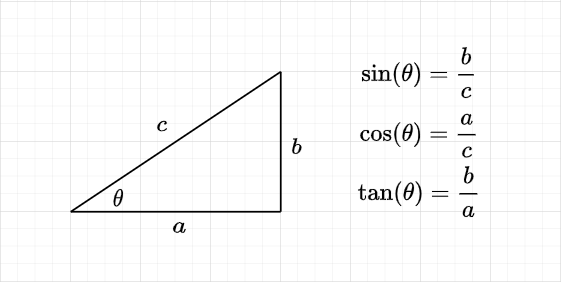
\includegraphics[scale=0.4]{images/Trigonometry Functions.png}
    \end{center}
\end{frame}

\begin{frame}{廣義角}
    \begin{alertblock}{廣義角}
    只被定義在直角三角形上的三角函數,並不方便。 \\
    \vspace{5mm}
    我們用單位圓 (Unit Circle) 定義了除了 $0 \le \theta \le 90 \degree$ 的角度時,三角函數的值。
    \end{alertblock}
    \begin{center}
        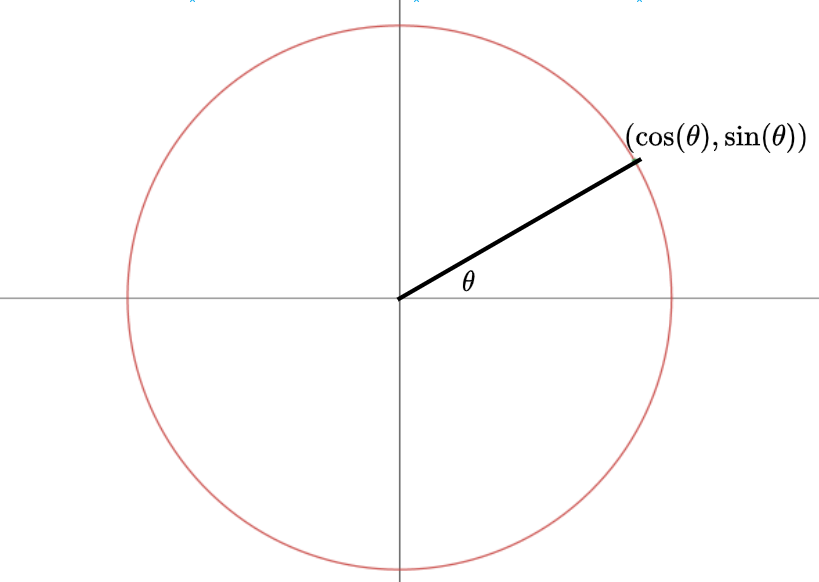
\includegraphics[scale=0.25]{images/unit circle.png}
    \end{center}
\end{frame}

\begin{frame}{弧度 (Radian)}
    由於角度 (Degree) 的使用,會導致在畫圖時的困擾,定義了另一個度數單位 - 弧度
    \begin{alertblock}{弧度 (Radian)}
        定義 $\pi$ 為 $180 \degree$,$2\pi$ 為 $360 \degree$ \\
        $$1 \text{ rad} = \frac{180}{\pi}\degree$$
        $$1 \degree = \frac{\pi}{180} \text{ rad}$$
    \end{alertblock}
    在 C++ 內建的三角函數 $\mathtt{sin(theta)}$, $\mathtt{cos(theta)}$, $\mathtt{tan(theta)}$ 都必須要使用弧度
\end{frame}

\begin{frame}{反三角函數 (Inverse Trigonometric Function)}
    \begin{alertblock}{反三角函數 (Inverse Trigonometric Function)}
        有了 $\sin(\theta)$, $\cos(\theta)$, $\tan(\theta)$ 的值,但想要知道 $\theta$ \\
        \vspace{5mm}
        $\arcsin(x) = \sin^{-1}(x)$: $0 \le x \le 1, \ -\dfrac{\pi}{2} \le \sin^{-1}(x) \le \dfrac{\pi}{2}$ \\
        \vspace{2.5mm}
        $\arccos(x) = \cos^{-1}(x)$: $0 \le x \le 1, \ 0 \le \cos^{-1}(x) \le \pi$ \\
        \vspace{2.5mm}
        $\arctan(x) = \tan^{-1}(x)$: $-\dfrac{\pi}{2} \le \tan^{-1}(x) \le \dfrac{\pi}{2}$
    \end{alertblock}
    在 C++ 中,想要知道 $\pi$,可以直接呼叫 $\mathtt{acos(-1)}$ \\
    \vspace{2.5mm}
    順道一提,\texttt{atan2(y,x) = atan(y/x)},而 $-\pi \le atan2(y,x) \le \pi$
\end{frame}

\section{高中數學複習 - 向量}

\begin{frame}{什麼是向量?}
    \begin{itemize}
        \item<1-> 同時有方向和大小的量
        \item<2-> 表示方式:
        \begin{itemize}
            \item 直接將向量畫出來
        \end{itemize}
        \begin{center}
            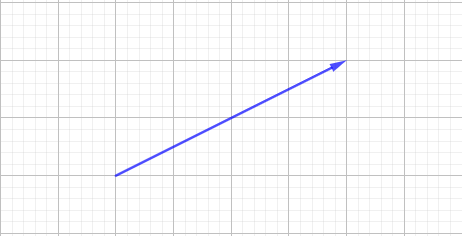
\includegraphics[scale=0.5]{images/vector.png}
        \end{center}
    \end{itemize}
\end{frame}

\begin{frame}{什麼是向量?}
    \begin{itemize}
        \item 同時有方向和大小的量
        \item 表示方式:
        \begin{itemize}
            \item 寫成從起點 $A(x_1,y_1)$ 指到終點 $B(x_2,y_2)$ 的向量,表示為 $\overrightarrow{AB} = (x_2-x_1,y_2-y_1)$
        \end{itemize}
        \begin{center}
            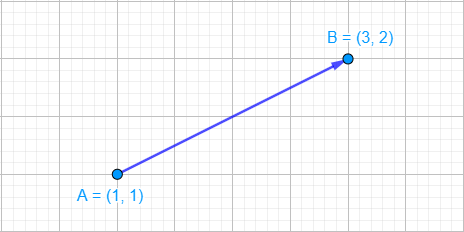
\includegraphics[scale=0.5]{images/Two Points Form.png}
        \end{center}
    \end{itemize}
\end{frame}

\begin{frame}{什麼是向量?}
    \begin{itemize}
        \item 向量 (Vector),同時有方向和大小的量
        \item 表示方式:
        \begin{itemize}
            \item 寫成從原點 $O(0,0)$ 指到終點 $A(x_1,y_1)$ 的向量,表示為 $\overrightarrow{A} = (x_1,y_1)$
        \end{itemize}
        \begin{center}
            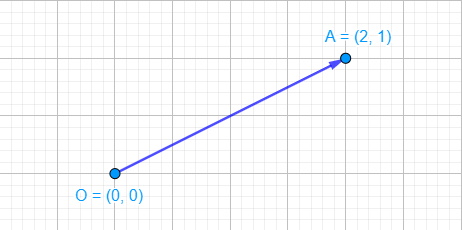
\includegraphics[scale=0.5]{images/vector_from_O.png}
        \end{center}
    \end{itemize}
\end{frame}

\begin{frame}{什麼是向量?}
    \begin{itemize}
        \item 向量的維度可以是很多維,但最常用的是二維(平面)與三維(空間)的形式
        \item 可以想成是兩點在空間中的位移
        \item 一個向量由其方向(單位向量)與大小所決定
    \end{itemize}
\end{frame}

\begin{frame}{什麼是向量?}
    \begin{alertblock}{向量的大小 (Magnitude)}
        又稱長度、模長。一個 $n$ 維向量 $\vec v = (x_1,x_2,\dots,x_n)$ 的大小為 $|\vec v| = \sqrt{x_1^2+x_2^2+\dots+x_n^2}$
    \end{alertblock}
    \begin{center}
        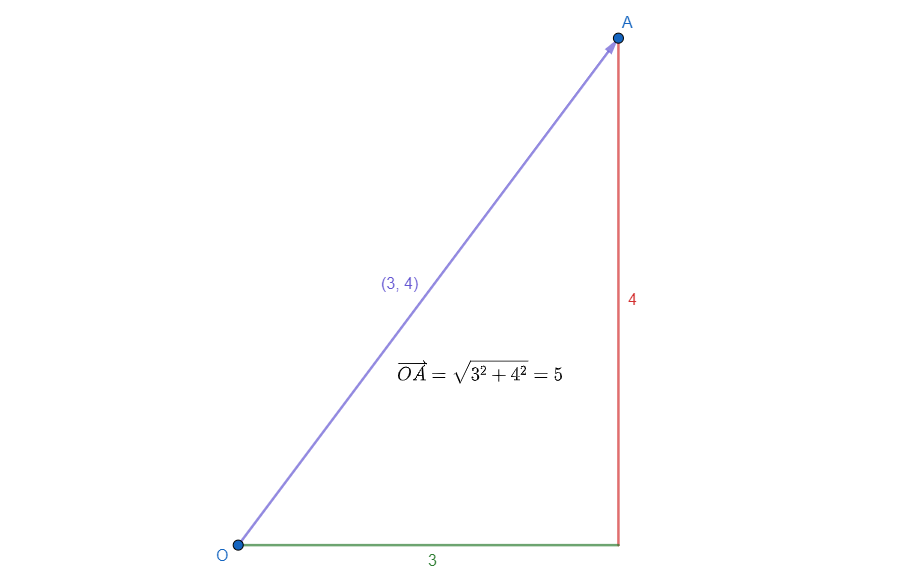
\includegraphics[scale=0.3]{images/magnitude.png}
    \end{center}
\end{frame}

\begin{frame}{什麼是向量?}
    \begin{alertblock}{單位向量 (Unit Vector)}
        大小為 $1$ 的向量。單位向量決定了向量的方向。\\
        \vspace{5mm}
        對於任一個 $n$ 維向量 $\vec v = (x_1,x_2,\dots,x_n)$,皆可以找到一個與其同向的單位向量 $\frac{\vec v}{|v|}$
    \end{alertblock}
    \begin{center}
        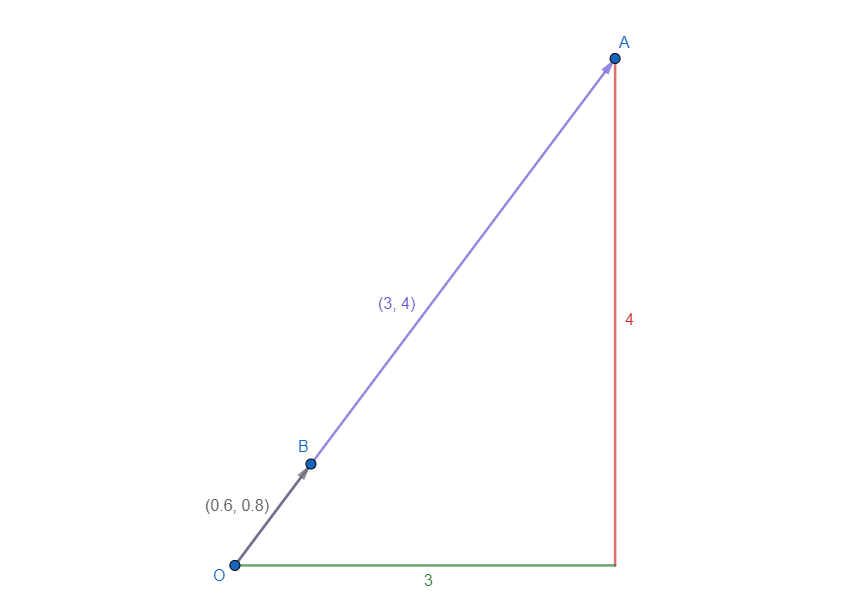
\includegraphics[scale=0.25]{images/unit vector.png}
    \end{center}
\end{frame}

\begin{frame}{向量運算}
    \begin{alertblock}{向量的加法 (Vector Addition)}
        對於兩個 $n$ 維向量 $\vec a = (a_1,a_2,\dots,a_n), \ \vec b = (b_1,b_2, \dots, b_n)$ \\
        \vspace{2.5mm}
        定義 $\vec a + \vec b = (a_1+b_1,a_2+b_2,\dots,a_n+b_n)$,可以使用平行四邊形法則畫出來
    \end{alertblock}
    \begin{center}
        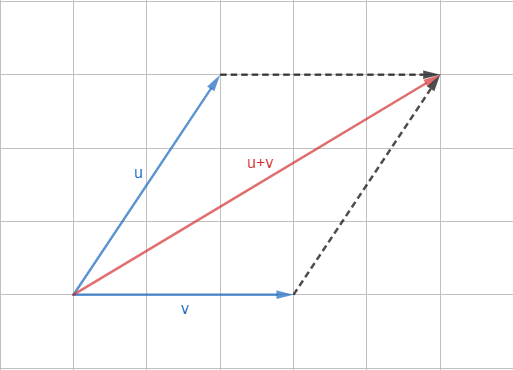
\includegraphics[scale=0.45]{images/vector_addition.png}
    \end{center}
\end{frame}

\begin{frame}{向量運算}
    \begin{alertblock}{純量乘法 (Scalar Multiplication)}
        對於一個 $n$ 維向量 $\vec a = (a_1,a_2,\dots,a_n)$,以及一個純量 $c$ \\
        \vspace{2.5mm}
        定義 $c \vec a = (ca_1,ca_2,\dots,ca_n)$,等同大小放大了 $c$ 倍
    \end{alertblock}
    \begin{center}
        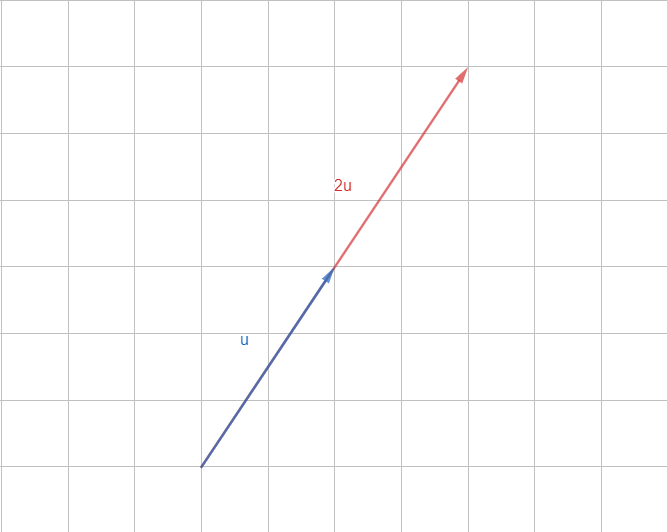
\includegraphics[scale=0.3]{images/scalar_multiplication.png}
    \end{center}
\end{frame}

\begin{frame}{向量運算}
    \begin{alertblock}{向量內積 (Dot Product)}
        對於兩個 $n$ 維向量 $\vec a = (a_1,a_2,\dots,a_n), \ \vec b = (b_1,b_2, \dots, b_n)$ \\
        \vspace{2.5mm}
        定義 $\vec a \cdot \vec b = a_1b_1+a_2b_2+\dots+a_nb_n$。等同於 $\vec b$ 投影到 $\vec a$ 的長度乘以 $\vec a$ 的長度 \\
        \vspace{2.5mm}
        $$\vec a \cdot \vec b = |\vec a| |\vec b| \cos \theta$$
    \end{alertblock}
    \begin{center}
        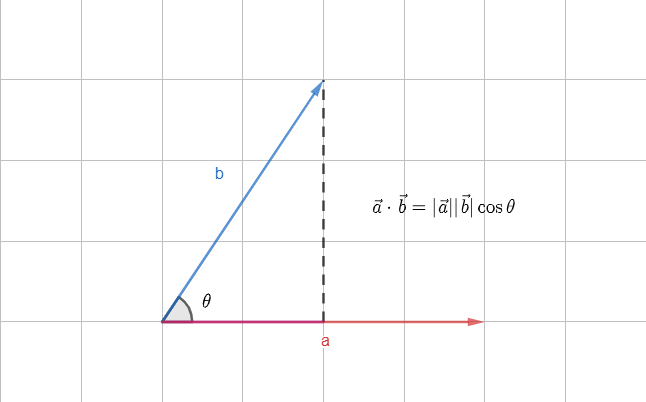
\includegraphics[scale=0.3]{images/dot_product.png}
    \end{center}
\end{frame}

\begin{frame}{向量運算}
    \begin{alertblock}{向量外積 (Cross Product)}
        對於兩個 $3$ 維向量 $\vec a = (a_1,a_2,a_3), \ \vec b = (b_1,b_2,b_3)$ \\
        \vspace{2.5mm}
        定義 $\vec a \times \vec b$ 為一個與 $\vec a$ 和 $\vec b$ 同時垂直的向量 $\vec c$ \\
        \vspace{2.5mm}
        計算方式為
        $$\begin{vmatrix} i & j & k \\ a_1 & a_2 & a_3 \\ b_1 & b_2 & b_3 \end{vmatrix}$$
        特點是 $|\vec a \times \vec b| = |\vec a| |\vec b| \sin \theta$ 等同於 $\vec a$ 與 $\vec b$ 所夾的平行四邊形面積 \\
        \vspace{2.5mm}
        可以使用右手定則判斷外積出來的向量方向。
    \end{alertblock}
\end{frame}

\begin{frame}{向量運算}
    \begin{alertblock}{向量外積 (Cross Product)}
        儘管外積的定義只有在三維向量,在程式中,我們通常只會用到二維的向量。 \\
        \vspace{2.5mm}
        因此在程式中,我們通常定義 $\vec a \times \vec b$ 是一個純量,而面積的正負表示方向 \\
        \vspace{2.5mm}
        定義 $\vec a \times \vec b = |\vec a| |\vec b| \sin \theta = a_1b_2 - a_2b_1$
    \end{alertblock}
    \begin{figure}
    \subfigure{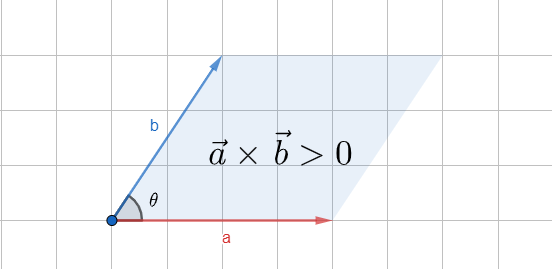
\includegraphics[width=5cm]{images/cross_product.png}}
    \hspace{5mm}
    \subfigure{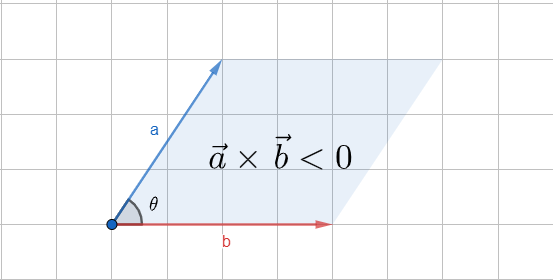
\includegraphics[width=5cm]{images/cross_product_2.png}}
    \end{figure}
\end{frame}

\begin{frame}{向量運算}
    \begin{alertblock}{向量之間的夾角}
        我們可以根據內積的定義 $\vec a \cdot \vec b = |\overrightarrow{a}| |\overrightarrow{b}| \cos \theta$ 來得到
        $$\theta = \cos^{-1}(\frac{\vec a \cdot \vec b}{|\overrightarrow{a}| |\overrightarrow{b}|})$$
    \end{alertblock}
\end{frame}

\section{用電腦存向量}

\begin{frame}{怎麼在程式中實作向量?}
    以下是在打比賽時常見的作法
    \begin{itemize}
        \item 為了方便起見,將所有向量儲存成從原點開始的向量 (用點 $A$ 的位置 $(x,y)$ 表示 $\overrightarrow{OA}$)
        \item 常見實作方式是使用 \texttt{pair<int,int>}, \texttt{pair<double,double>} 或者 \texttt{struct}
        \item 通常會將向量寫成模板
    \end{itemize}
\end{frame}

\begin{frame}{怎麼在程式中實作向量?}
    \lstinputlisting[language=C++]{point.cpp}
\end{frame}

\begin{frame}[fragile]{怎麼在程式中實作向量?}
    剛剛的程式碼中,出現了這個函式 \texttt{sign()},而這個函式是幫助我們在浮點數時判斷正負的
    \begin{lstlisting}[language=C++, basicstyle=\ttfamily\small]
int sign(double a){
    if(abs(a) < EPS) return 0;
    else return (a > 0 ? 1 : -1);
}
    \end{lstlisting}
    EPS 的估計,我們會在這堂課後面與大家介紹,不過通常取 $10^{-6}$, $10^{-7}$ 就足夠了
\end{frame}

\begin{frame}[fragile]{怎麼在程式中實作向量?}
    判斷順時針與逆時針,我們可以使用剛剛的 \texttt{ori(a,b,c)} 來做到 \\
    \vspace{5mm}
    概念是,我們想要判斷 $\overrightarrow{AB}$ 轉到 $\overrightarrow{BC}$ 是順時針還是逆時針 
    \begin{center}
        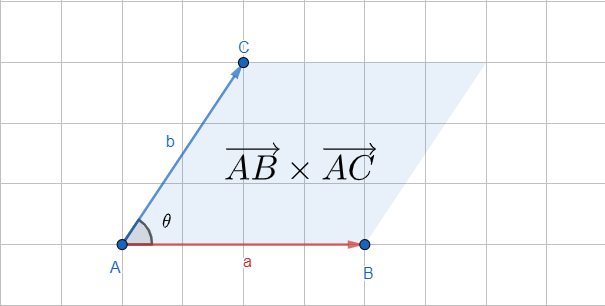
\includegraphics[scale=0.5]{images/ori.png}
    \end{center}
    直接使用外積即可
\end{frame}

\section{浮點數誤差分析}

\begin{frame}[fragile]{浮點數在電腦中的儲存}
    \begin{alertblock}{IEEE 754}
        浮點數在電腦中的儲存被分成三個部分,\texttt{sign}, \texttt{exponent}, \texttt{significand}
        $$\mathtt{value} = -1^{\mathtt{sign}} \times 2^{\mathtt{exponent}} \times \mathtt{significand}$$
        \texttt{sign} 表示了浮點數的正負號 \\
        \vspace{2.5mm}
        \texttt{exponent} 與 \texttt{significand} 表示了科學記號的形式 \\
        \vspace{2.5mm}
        \texttt{significand} 是一個介於 $1$ 到 $2$ 之間的數字,例如: $\mathtt{1.0101} = 2^0 + 2^{-2} + 2^{-4} = 1.3125$
    \end{alertblock}
    \begin{center}
        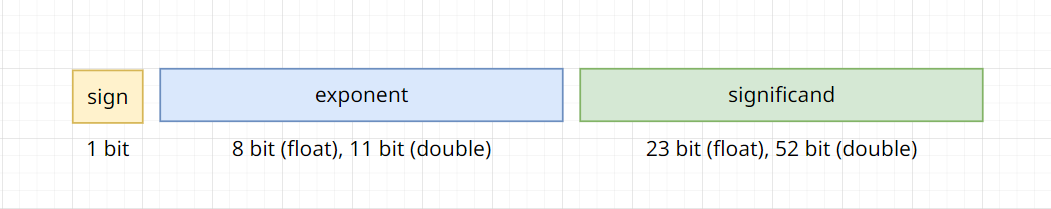
\includegraphics[scale=0.3]{images/IEEE754.png}
    \end{center}
\end{frame}

\begin{frame}[fragile]{浮點數在電腦中的儲存}
    \begin{alertblock}{浮點數誤差}
        正如同我們無法使用十進位的小數完整表示 $\frac{1}{3}, \ \frac{1}{7}$ 等數字 \\
        \vspace{2.5mm}
        在電腦中,我們也只能想辦法使用二進位來逼近一個數字\\
        \vspace{2.5mm}
        因此,在大部分的浮點數運算,數字一定會出現誤差
    \end{alertblock}
\end{frame}

\begin{frame}[fragile]{浮點數在電腦中的儲存}
    以下是 C++ 不同型態在儲存浮點數時,會產生的相對誤差 \\
    \vspace{2.5mm}
    \begin{center}
        \begin{tabular}{|c|c|c|}
            \hline
            Type & Size &  Relative Precision \\ \hline \hline
            \texttt{float} & 4 Bytes & $2^{-23} \approx 10^{-7}$ \\ \hline 
            \texttt{double} & 8 Bytes & $2^{-52} \approx 10^{-16}$ \\ \hline
            \texttt{long double} & 10 Bytes & $2^{-63} \approx 10^{-19}$ \\ \hline
        \end{tabular}
    \end{center}
\end{frame}

\begin{frame}[fragile]{絕對誤差與相對誤差}
    通常在競程中會遇到的題目,都會出現 「絕對誤差或相對誤差不超過 $\epsilon$ 就算正確」
    \begin{alertblock}{絕對誤差 (Absolute Error)}
        計算出的答案 $x$ 與正確答案 $\mathtt{ans}$ 的差 $|x - \mathtt{ans}|$
    \end{alertblock}
    
    \begin{alertblock}{相對誤差 (Relative Error)}
        絕對誤差與正確答案的比例 $\frac{\mathtt{absolute} \ \mathtt{error}}{\mathtt{ans}}$
    \end{alertblock}
\end{frame}

\begin{frame}[fragile]{誤差的傳遞}
    當我們在進行浮點數運算時,儘管數字一開始的誤差很小,經過運算後,誤差會逐漸累計
    \begin{alertblock}{加減法運算}
        在加減法運算時,最差的情況,絕對誤差會變成兩數絕對誤差之和
        $$(x+\Delta x) \pm (y + \Delta y) = (x \pm y) + (\Delta x \pm \Delta y)$$
    \end{alertblock}
\end{frame}

\begin{frame}[fragile]{誤差的傳遞}
    當我們在進行浮點數運算時,儘管數字一開始的誤差很小,經過運算後,誤差會逐漸累計
    \begin{alertblock}{乘除法運算}
        在乘運算時,最差的情況,相對誤差會變成兩數相對誤差之和
        $$(x+\Delta x)(y + \Delta y) = xy(1 + \frac{\Delta x}{x})(1 + \frac{\Delta y}{y}) \approx xy(1+ \frac{\Delta x}{x} + \frac{\Delta y}{y})$$
    \end{alertblock}
\end{frame}

\begin{frame}[fragile]{誤差的傳遞}
    根據剛剛的兩個結論,通常如果我們要估計誤差,如果我們做了 $N$ 次的運算 \\
    \vspace{2.5mm}
    其相對誤差不會超過 $N \epsilon$,因此可以使用這樣的方式去估計誤差,並決定 \texttt{EPS} 的大小
\end{frame}

\section{向量的應用}

\begin{frame}[fragile]{三點共線}
    現在你有三個點 $A, \ B, \ C$,要如何判斷這三個點是否共線呢?
    \begin{center}
        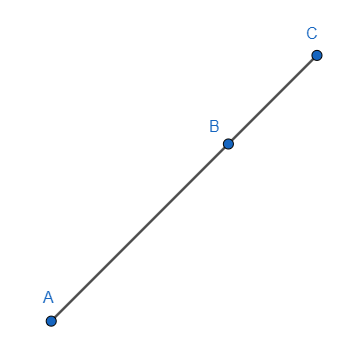
\includegraphics[scale=0.6]{images/colinear.png}
    \end{center}
\end{frame}

\begin{frame}[fragile]{三點共線}
    一個沒學過向量的人,常用的方法可能是分別找出兩點之間直線的斜率。 \\
    \vspace{5mm}
    不過,我們現在有了向量的知識,其實只要 $\overrightarrow{AB}$ 與 $\overrightarrow{AC}$ 同向即可 \\
    \begin{lstlisting}[language=C++,basicstyle=\ttfamily\small]
bool colinear(point a, point b, point c){
    return sign((b-a)^(c-a)) == 0;
}
    \end{lstlisting}
    可以使用交叉相乘,或者直接用外積判斷 $\overrightarrow{AB} \times \overrightarrow{AC} = 0$ ($\overrightarrow{AB}$ 與 $\overrightarrow{AC}$ 夾成的面積為 $0$)
\end{frame}

\begin{frame}[fragile]{點是否在線段上}
    現在你有三個點 $A, \ B, \ C$,要如何判斷 $C$ 是否在 $\overline{AB}$ 上呢?
    \begin{center}
        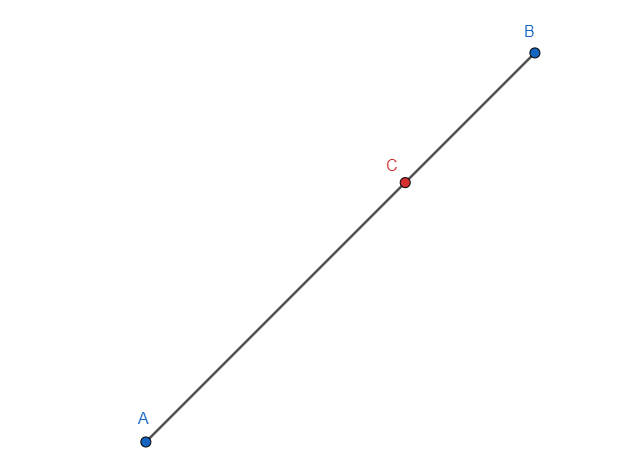
\includegraphics[scale=0.5]{images/between.png}
    \end{center}
\end{frame}

\begin{frame}[fragile]{點是否在線段上}
    只要滿足兩個條件,$C$ 就會在 $\overline{AB}$ 上了
    \begin{enumerate}
        \item $A,B,C$ 三點共線
        \item $\overrightarrow{CA}, \ \overrightarrow{CB}$ 反向
    \end{enumerate} \pause
    如何判斷兩個向量是否反向呢? \pause 內積 $< 0$
\end{frame}

\begin{frame}[fragile]{點是否在線段上}
    只要滿足兩個條件,$C$ 就會在 $\overline{AB}$ 上了
    \begin{enumerate}
        \item $A,B,C$ 三點共線
        \item $\overrightarrow{CA}, \ \overrightarrow{CB}$ 反向
    \end{enumerate}
    如何判斷兩個向量是否反向呢? 內積 $< 0$
    
    \begin{lstlisting}[language=C++,basicstyle=\ttfamily\small]
bool between(point a, point b, point c){
    if(!colinear(a,b,c)) return false;
    return sign((a-c) * (b-c)) <= 0; 
}
    \end{lstlisting}
\end{frame}

\begin{frame}[fragile]{線段相交}
    現在你有兩個線段 $\overline{AB}$ 與 $\overline{CD}$,要怎麼判斷兩線段是否相交?
    \begin{center}
        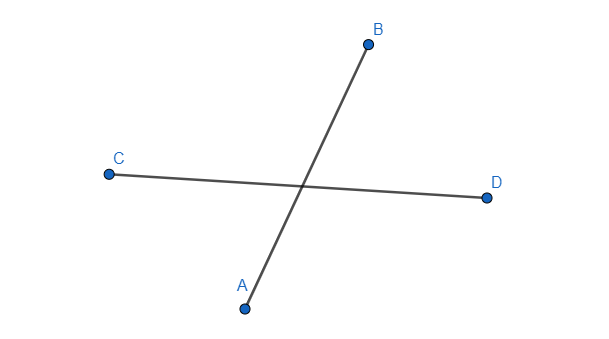
\includegraphics[scale=0.5]{images/segment_intersect.png}
    \end{center}
\end{frame}

\begin{frame}[fragile]{線段相交}
    $C,D$ 對於 $\overline{AB}$ 必須在兩側,$A,B$ 對於 $\overline{CD}$ 也必須在兩側 \\
    \vspace{5mm}
    滿足 $(\overrightarrow{AB} \times \overrightarrow{AC})(\overrightarrow{AB} \times \overrightarrow{AD}) < 0$ 且 $(\overrightarrow{CD} \times \overrightarrow{CA})(\overrightarrow{CD} \times \overrightarrow{CB}) < 0$ \\
    \vspace{5mm}
    但是,有沒有別的可能性呢?
\end{frame}

\begin{frame}[fragile]{線段相交}
    $\overline{AB}$ 與 $\overline{CD}$ 兩線段平行怎麼辦? \pause
    \begin{figure}
    \subfigure{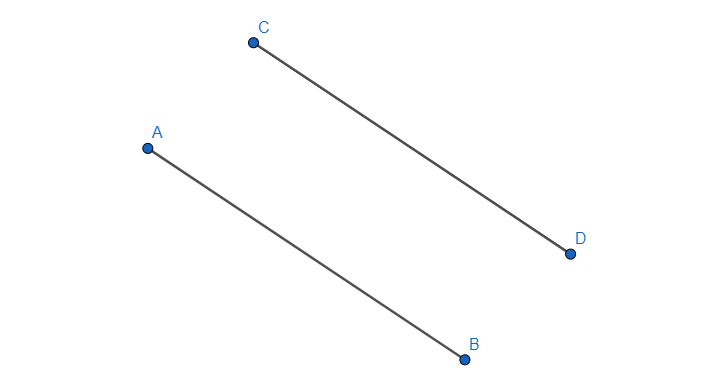
\includegraphics[width=5cm]{images/intersect_parallel.png}}
    \hspace{5mm}
    \subfigure{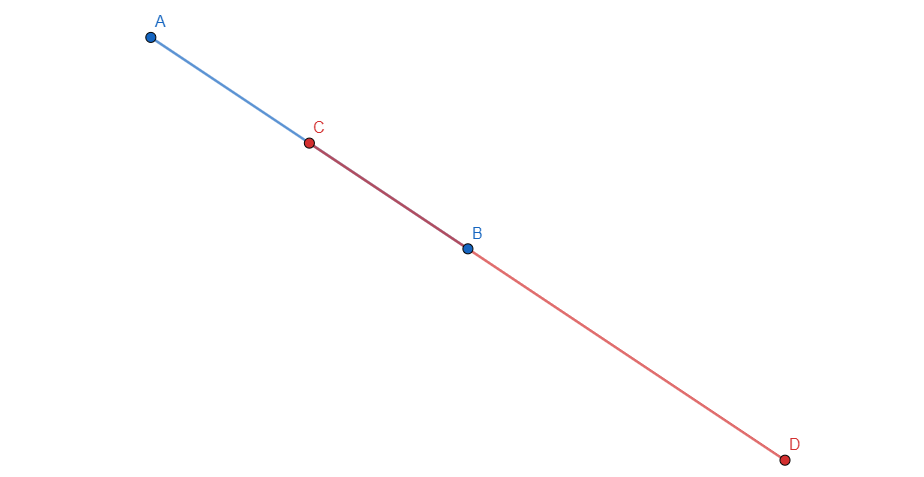
\includegraphics[width=5cm]{images/intersect_parallel_2.png}}
    \end{figure}
    會發生 $(\overrightarrow{AB} \times \overrightarrow{AC}) = 0$ 且 $(\overrightarrow{AB} \times \overrightarrow{AD}) = 0$ 的情況,判斷點是否互相在對方的線段上即可
\end{frame}

\begin{frame}[fragile]{線段相交}
    這裡的函數有人會叫 \texttt{intersect()} 也有人會叫香蕉 \texttt{banana()}
    \begin{lstlisting}[language=C++,basicstyle=\ttfamily\small]
bool intersect(point a, point b, point c, point d){
    int abc = ori(a,b,c);
    int abd = ori(a,b,d);
    int cda = ori(c,d,a);
    int cdb = ori(c,d,b);
    if(abc==0 && abd==0) 
        return between(a,b,c) || between(a,b,d) || between(c,d,a) || between(c,d,b);
    return abc * abd <= 0 && cda * cdb <= 0;
}
    \end{lstlisting}
\end{frame}

\begin{frame}[fragile]{線段交點}
    現在你有兩個線段 $\overline{AB}$ 與 $\overline{CD}$,要怎麼計算兩線段交點 $P$?
    \begin{center}
        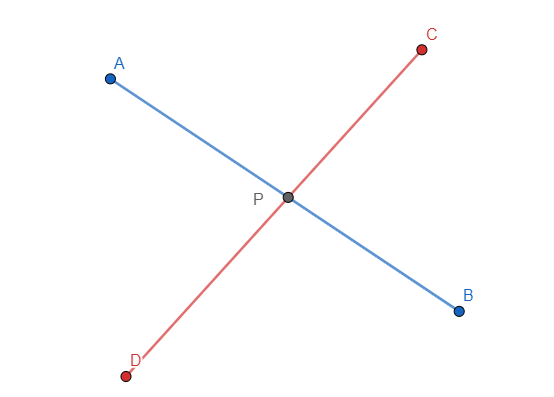
\includegraphics[scale=0.5]{images/intersect_point.png}
    \end{center}
\end{frame}

\begin{frame}[fragile]{線段交點}
    高中的時候有學過分點公式,我們可以使用面積比例套分點公式計算出交點位置
    \begin{center}
        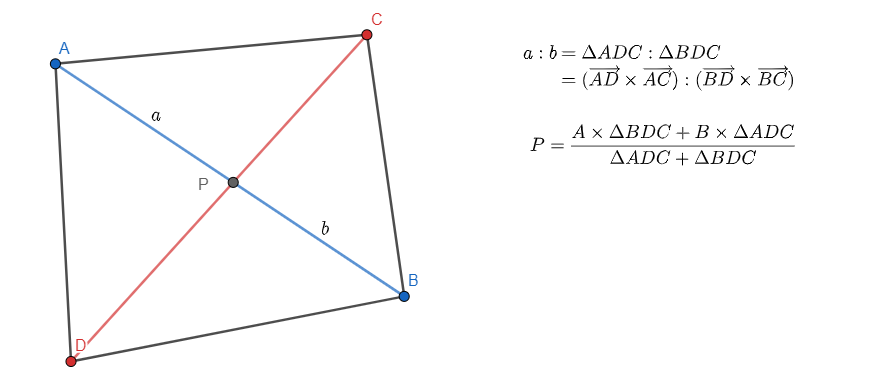
\includegraphics[scale=0.5]{images/intersect_point_2.png}
    \end{center}
\end{frame}

\begin{frame}[fragile]{線段交點}
    這個方法只要在兩線段不平行時,都能計算出答案,包含兩線段延伸出去的交點
    \begin{lstlisting}[language=C++,basicstyle=\ttfamily\small]
point intersect_point(point a, point b, point c, point d){
    int adc = (d-a) ^ (c-a);
    int bdc = (d-b) ^ (b-a);
    return (a * bdc + b * adc) / (adc + bdc);
}
    \end{lstlisting}
\end{frame}

\begin{frame}[fragile]{投影}
    現在你有一個三個點 $A,B,C$,請找到 $\overrightarrow{AC}$ 投影在 $\overrightarrow{AB}$ 上的向量
    \begin{center}
        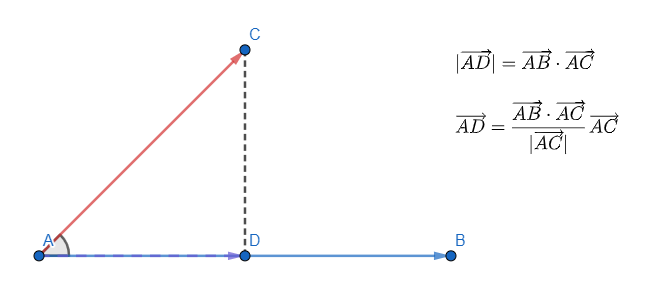
\includegraphics[scale=0.5]{images/projection.png}
    \end{center}
\end{frame}

\begin{frame}[fragile]{投影}
    直接套正射影公式即可
    \begin{lstlisting}[language=C++,basicstyle=\ttfamily\small]
point projection(point a, point b, point c){
    return (c-a) * ((b-a) * (c-a)) / abs(c-a);
}
    \end{lstlisting}
\end{frame}

\begin{frame}{多邊形面積}
    照順序給你一個多邊形 $P_0 P_1\cdots P_{n-1}$的面積,請問這個多邊形的面積是多少?
    \begin{center}
        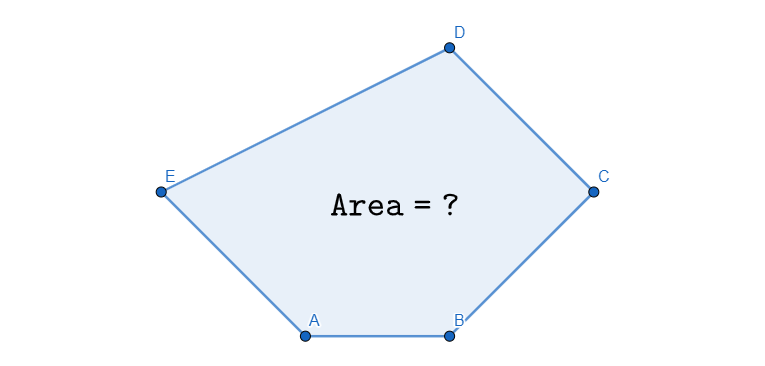
\includegraphics[scale=0.5]{images/polygon_area.png}
    \end{center}
\end{frame}

\begin{frame}{多邊形面積}
    \begin{itemize}
        \item 首先,我們知道 $\Delta ABC = \frac{1}{2}|\overrightarrow{AB} \times \overrightarrow{AC}|$ \item 則我們可以將多邊形想成是很多個三角形的面積相加 (面積可正可負)
        \item 令 $P_n = P_0$,面積就是 $\sum_{i=0}^{n-1} P_i \times P_{i+1}$
        \item 這個公式就是廣為人知的「測量師公式」或「鞋帶公式」
        \item 不只凸多邊形可以用,凹的也可以
    \end{itemize}
\end{frame}

\begin{frame}{點是否在多邊形內部}
    照順序給你一個多邊形 $P_0 P_2\cdots P_{n-1}$,還有一個點 $A$,請問 $A$ 是否在多邊形內部?
    \begin{center}
        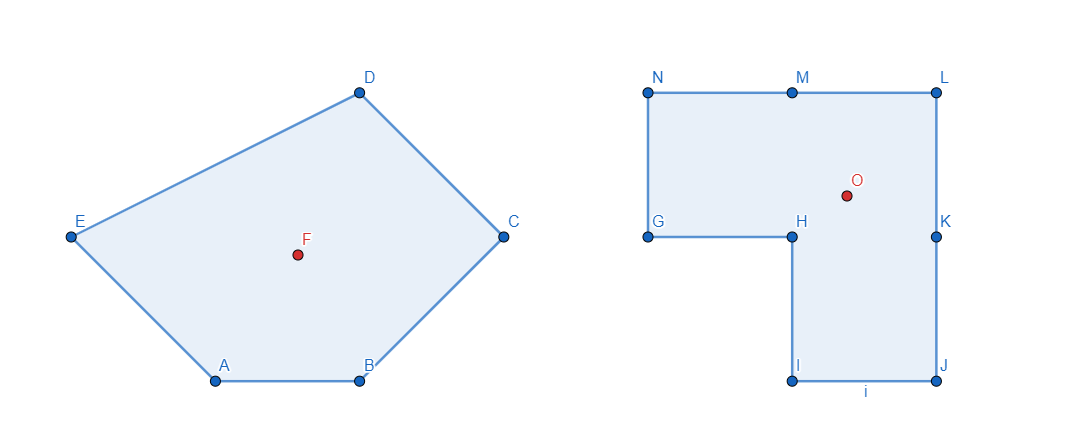
\includegraphics[scale=0.5]{images/point_in_polygon.png}
    \end{center}
\end{frame}

\begin{frame}{點是否在多邊形內部}
    這個問題有個很經典的處理方式,我們可以從 $A$ 點開始,往外射出一條射線 \\
    \vspace{2.5mm}
    一個點是否在多邊形內部 $\iff$ 射出去的射線與奇數個多邊形的邊相交\\
    \vspace{2.5mm}
    判斷時,要注意射線會不會打到頂點,否則答案可能會算錯
    \begin{center}
        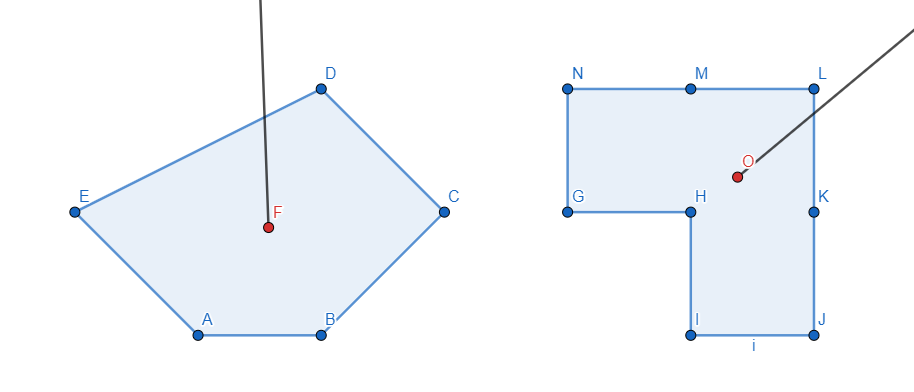
\includegraphics[scale=0.5]{images/point_in_polygon_2.png}
    \end{center}
\end{frame}

\begin{frame}{練習題}
    \begin{block}{CSES - Point Location Test}
        檢查一個點在線段左邊、右邊、還是在上面
    \end{block}
    \begin{block}{CSES - Line Segment Intersection}
        給你兩個線段,檢查兩個線段是否相交
    \end{block}
    \begin{block}{CSES - Polygon Area}
        給你多邊形的點,找到多邊形的面積
    \end{block}
\end{frame}

\section{凸包 (Convex Hull)}

\begin{frame}{什麼是凸包?}
    對於平面上的點集,找到一個包含所有點的最小凸多邊形,這個凸多邊形即為凸包
    \begin{center}
        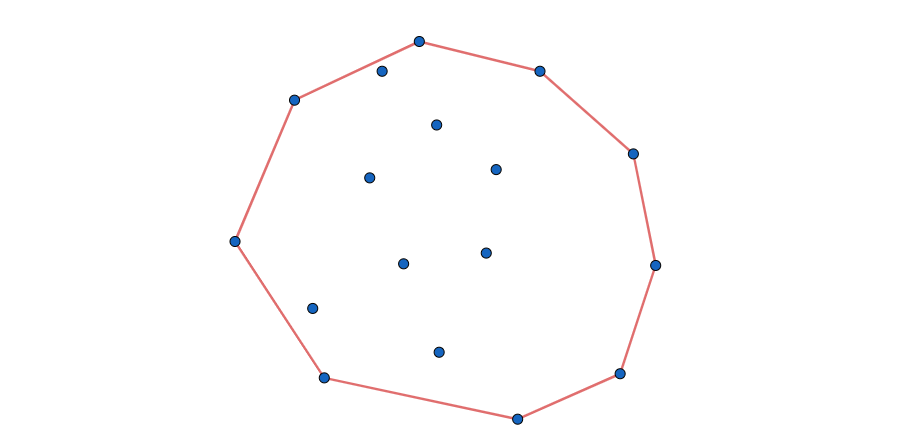
\includegraphics[scale=0.5]{images/convex_hull.png}
    \end{center}
\end{frame}

\begin{frame}{要怎麼找凸包?}
    比較廣為人知的兩種凸包演算法是「Monotone Chain」和「Graham Scan」 \\
    \vspace{2.5mm}
    其中,第一種的 Monotone Chain 是在打競程比賽中較常被使用的演算法 \\
    \vspace{2.5mm}
    而第二種的 Graham Scan 則是用到了等等會教的極角排序。\\
    \vspace{2.5mm}
    不過在此,我們只會介紹第一種方法。
\end{frame}

\begin{frame}[fragile]{Monotone Chain}
    首先,先將點依照 $x$ 座標排序,相同的話,照 $y$ 進行排序
    \begin{lstlisting}[language=C++,basicstyle=\ttfamily\small]
bool operator < (point b){
    return a.x == b.x ? a.y < b.y : a.x < b.x;
}
    \end{lstlisting} \pause
    接著,我們依序去考慮每個點,類似在維護單調隊列的過程
    \begin{center}
        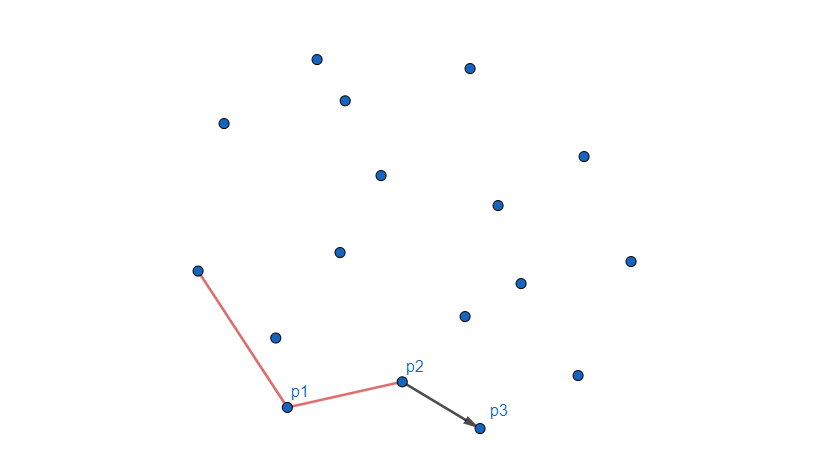
\includegraphics[scale=0.3]{images/monotone_chain_1.png}
    \end{center}
\end{frame}

\begin{frame}[fragile]{Monotone Chain}
    如果目前,在單調隊列最後的兩個點 $P_1, \ P_2$,與目前要新加入的點 $P_3$ \\
    \vspace{2.5mm}
    如果 $\overrightarrow{P_1P_3} \times \overrightarrow{P_1P_2} < 0$,則會導致多邊形不是凸的!
    \begin{center}
        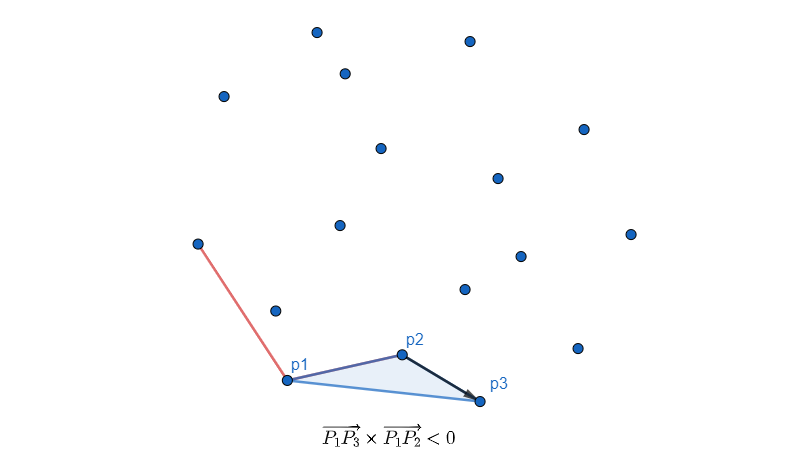
\includegraphics[scale=0.3]{images/monotone_chain_2.png}
    \end{center}
    遇到這種情況時,我們就必須要把 $P_2$ 給 pop 掉!
\end{frame}

\begin{frame}[fragile]{Monotone Chain}
    因此,原本的單調隊列就會將 $P_2$ 給移除,再一路用同樣的方式去處理即可
    \begin{center}
        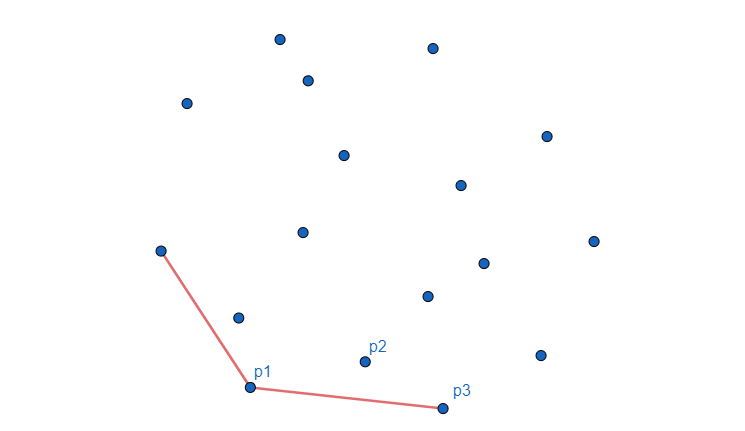
\includegraphics[scale=0.3]{images/monotone_chain_3.png}
    \end{center}
\end{frame}

\begin{frame}[fragile]{Monotone Chain}
    照著這樣的方式一路跑完,會建出 \textbf{下凸包}
    \begin{center}
        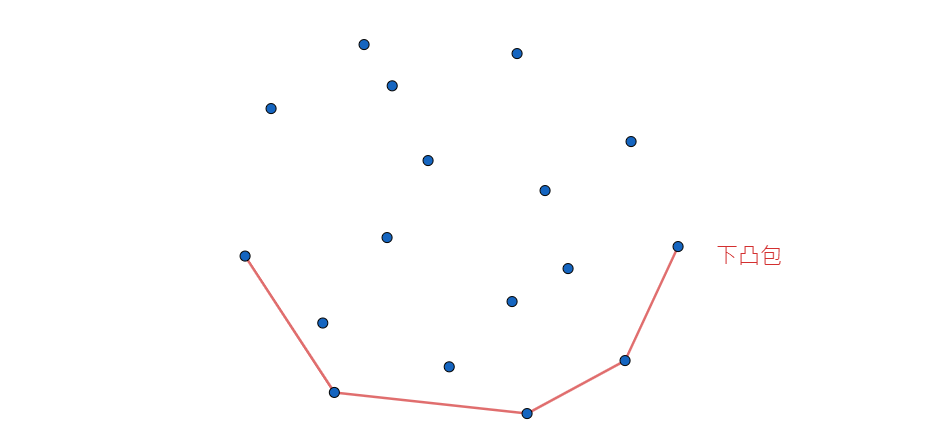
\includegraphics[scale=0.25]{images/bottom_convex_hull.png}
    \end{center} \pause
    只要把原來排序好的點,直接反轉過來,再做一次,就會得到上凸包!
    \begin{center}
        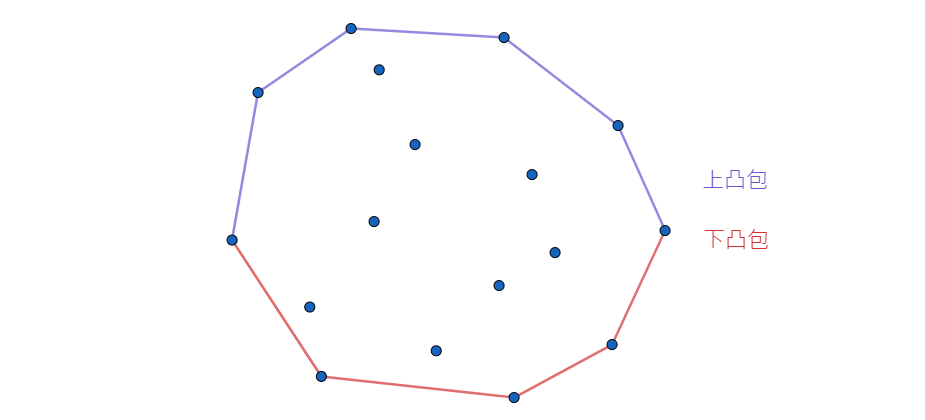
\includegraphics[scale=0.25]{images/upper_convex_hull.png}
    \end{center}
\end{frame}

\begin{frame}[fragile]{Monotone Chain}
    而這樣做,時間複雜度會是 $O(n \log n)$ (排序的時間複雜度)
    \begin{lstlisting}[language=C++,basicstyle=\ttfamily\tiny]
vector<point> convex_hull(vector<point> points){
    sort(points.begin(),points.end());

    vector<point> hull;
    for(int t = 0; t < 2; t++){
        int sz = hull.size();
        for(int i = 0; i < points.size(); i++){
            while(hull.size() >= sz+2 && ori(hull[hull.size()-2], hull.back(), points[i]) <= 0){
                hull.pop_back();
            }
            hull.push_back(points[i]);
        }
        hull.pop_back();
        reverse(points.begin(),points.end());
    }
    return hull;
}
    \end{lstlisting}
\end{frame}

\section{旋轉卡尺}

\begin{frame}[fragile]{旋轉卡尺的概念}
    首先,我們先看一題最經典的例題
    \begin{block}{最遠點對 (USACO 2003 - Beauty Contest G)}
        給你平面上的 $n$ 個點,請找到最遠點對之間的距離。\\
        \vspace{5mm}
        測資範圍: $1 \le n \le 5 \times 10^4$
    \end{block}
\end{frame}

\begin{frame}[fragile]{旋轉卡尺的概念}
    \begin{block}{最遠點對 (USACO 2003 - Beauty Contest G)}
        給你平面上的 $n$ 個點,請找到最遠點對之間的距離。\\
        \vspace{5mm}
        測資範圍: $1 \le n \le 5 \times 10^4$
    \end{block}
    最遠點對必定會出現在凸包的兩個點上,不過,我們要怎麼在凸包上找到最遠的兩個點呢? \\
    \vspace{2.5mm}
    雙指針!
\end{frame}

\begin{frame}[fragile]{旋轉卡尺的概念}
    旋轉卡尺 (Rotating Caliper),事實上可以想成兩個平行線,夾著一個凸多邊形進行旋轉
    \begin{center}
        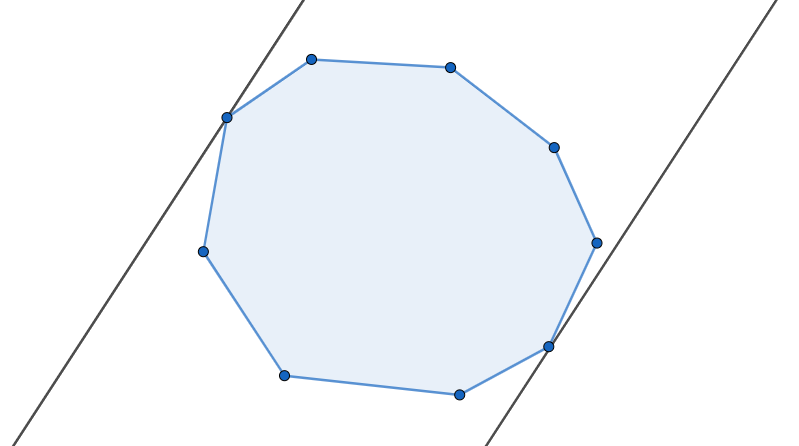
\includegraphics[scale=0.3]{images/rotating_caliper.png}
    \end{center}
\end{frame}

\begin{frame}[fragile]{旋轉卡尺的概念}
    不過,我們無法完全模擬旋轉的每個時刻,因此只會去計算直線是多邊形上的邊的情形
    \begin{center}
        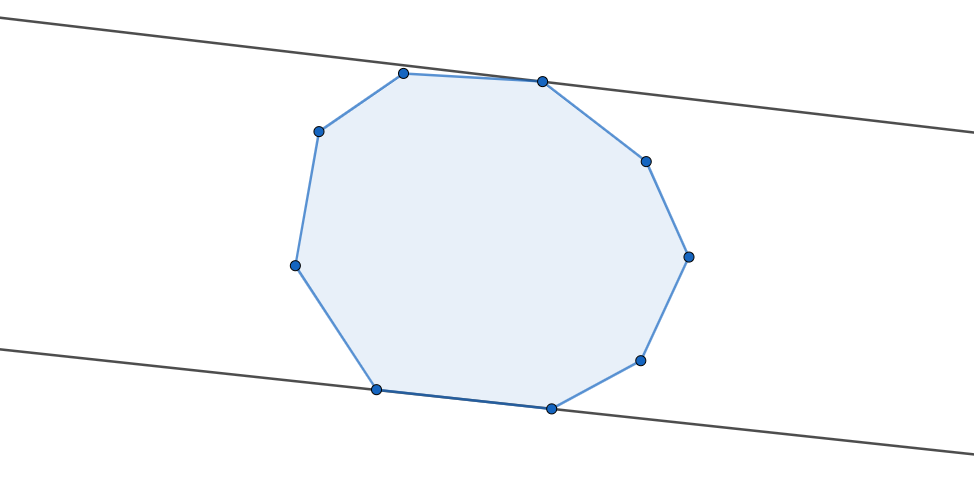
\includegraphics[scale=0.3]{images/rotating_caliper_2.png}
    \end{center}
\end{frame}

\begin{frame}[fragile]{旋轉卡尺的概念}
    當我們在枚舉平行線時,最遠點必定會出現在這條線段的最遠處
    \begin{center}
        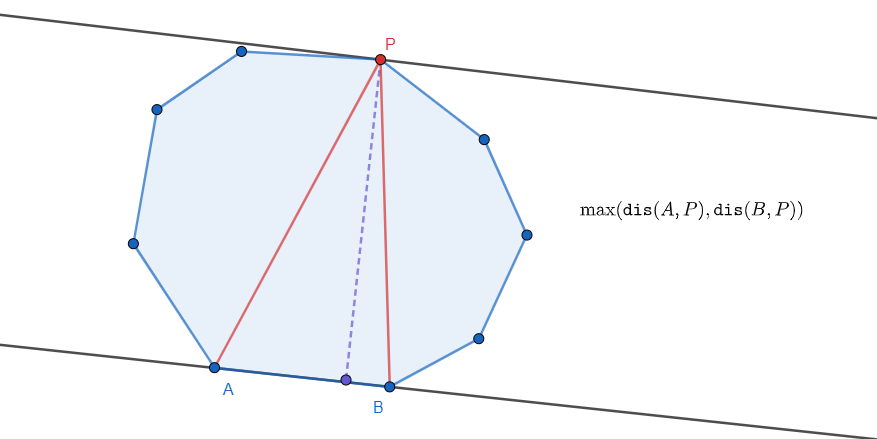
\includegraphics[scale=0.3]{images/farthest pair of points.png}
    \end{center}
    照著這樣的概念,我們只要對點找出凸包之後,再上面進行旋轉卡尺 (雙指針) 即可
\end{frame}

\begin{frame}[fragile]{旋轉卡尺的概念}
    以下是參考程式碼 (單純旋轉卡尺,複雜度是 $O(n)$)
    \begin{lstlisting}[language=C++,basicstyle=\ttfamily\tiny]
double farthest_pair_of_points(vector<point> hull){
    double res = 0;
    if(hull.size() == 2){
        return abs(hull[0]-hull[1]);
    }
 
    hull.push_back(hull[0]);
    
    int j = 2;
 
    for(int i = 0;i < hull.size()-1;i++){
        while(area(hull[i],hull[i+1],hull[j]) < area(hull[i],hull[i+1],hull[(j+1)%hull.size()])){
            j = (j+1)%hull.size();
        }
        res = max(res,max(abs(hull[i]-hull[j]),abs(hull[i+1]-hull[j])));
    }
 
    return res;
}
    \end{lstlisting}
\end{frame}

\section{極角排序}

\begin{frame}[fragile]{極角排序}
    在座標平面上有 $n$ 個點,要怎麼按照極角的順序將這些點排好呢?
    \begin{alertblock}{極角}
        從正 $x$ 方向開始,逆時針轉到 $(x,y)$ 時所需的角度 (極座標系的角度)
    \end{alertblock}
    \begin{center}
        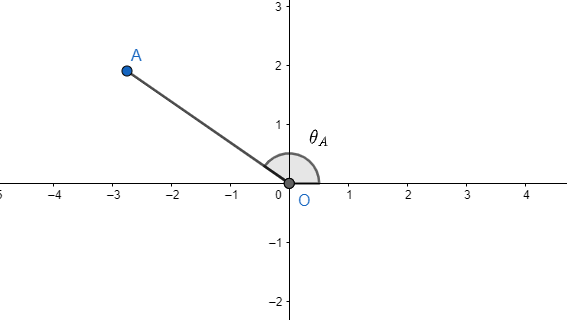
\includegraphics[scale=0.4]{images/polar_angle.png}
    \end{center}
\end{frame}

\begin{frame}[fragile]{極角排序}
    一個滿直覺的方式是使用 \texttt{atan2(y,x)} 的方式進行排序
    \begin{lstlisting}[language=C++,basicstyle=\ttfamily\small]
bool operator < (point b){
    return atan2(y,x) < atan2(b.y,b.x);
}
    \end{lstlisting}
    而這樣的方式,就可以快速的得到極角排序了 (不過象限順序是三四一二) \\
    \vspace{2.5mm}
    但由於 \texttt{atan2(y,x)} 會回傳浮點數,在某些情況,可能會導致精度產生問題 
\end{frame}

\begin{frame}[fragile]{極角排序}
    因此,我們希望可以有一個更好的排序方式。而我們提過,外積可以判斷兩個點的順逆時針關係
    \begin{center}
        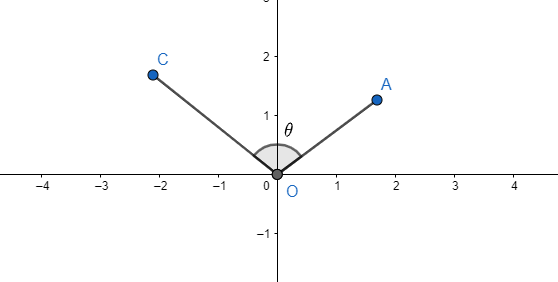
\includegraphics[scale=0.4]{images/polar_angle_sort.png}
    \end{center}
    以上圖為例,$A$ 對 $C$ 做外積結果為正,反之為負。 \\
    \vspace{2.5mm}
    因此,我們可以分一二象限與三四象限 (分成上下兩平面) 分別用外積排序即可
\end{frame}

\begin{frame}[fragile]{極角排序}
    使用外積的極角排序
    \begin{lstlisting}[language=C++,basicstyle=\ttfamily\small]
bool polar_sort(point a, point b){
    auto up = [&](point p){
        return p.y > 0 || p.y == 0 && p.x >= 0;
    };
    int A = up(a), B = up(b);

    if(A != B){
        return A < B;
    }

    if(sign(a^b) == 0)
        return abs(a) < abs(b);

    return sign(a^b) > 0;
}
    \end{lstlisting}
\end{frame}

\begin{frame}[fragile]{例題}
    \begin{block}{TOI 2020 初選 pD. 質感測試}
        在座標平面上有 $n$ 個燈泡,每個點有一個質感係數。而在 $(0,0)$ 上,有一根棒狀感應器。你可以選擇這個感應器初始的方向,問你最多可以讓感應器掃過的燈泡的質感係數總和為多少?
    \end{block}
    \begin{center}
        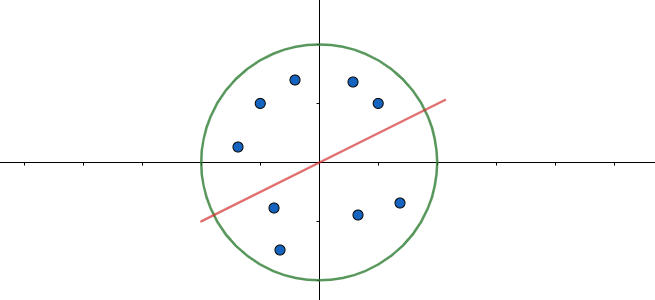
\includegraphics[scale=0.25]{images/tioj_2191.png}
    \end{center}
    \begin{center}
        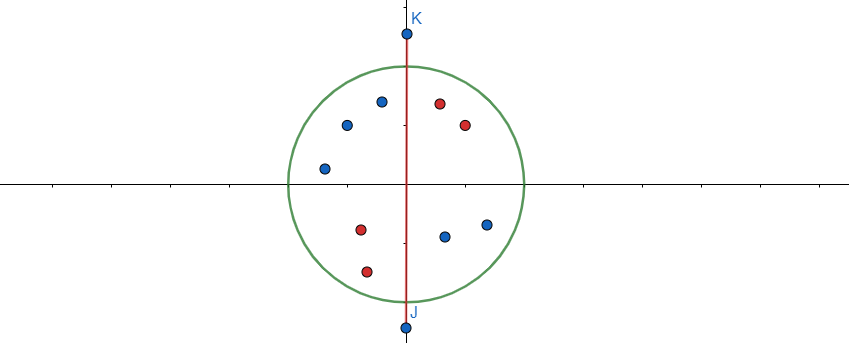
\includegraphics[scale=0.25]{images/tioj_2191_2.png}
    \end{center}
\end{frame}

\begin{frame}[fragile]{例題}
    \begin{block}{TOI 2020 初選 pD. 質感測試}
        在座標平面上有 $n$ 個燈泡,每個點有一個質感係數。而在 $(0,0)$ 上,有一根棒狀感應器。你可以選擇這個感應器初始的方向,問你最多可以讓感應器掃過的燈泡的質感係數總和為多少?
    \end{block}
    首先,觀察到感應器掃過的燈泡經過極角排序後,一定是連續的 \\ \pause
    我們只要將這些點進行極角排序之後 \\
    對陣列找「環狀最大連續和」即可 (環狀最大連續和 = \texttt{max(}最大連續和, 總和-最小連續和\texttt{)})
\end{frame}

\section{掃描線}

\begin{frame}{掃描線的概念}
    將幾何物件轉成不同的事件,使用掃描線的概念來進行枚舉,
    \begin{center}
        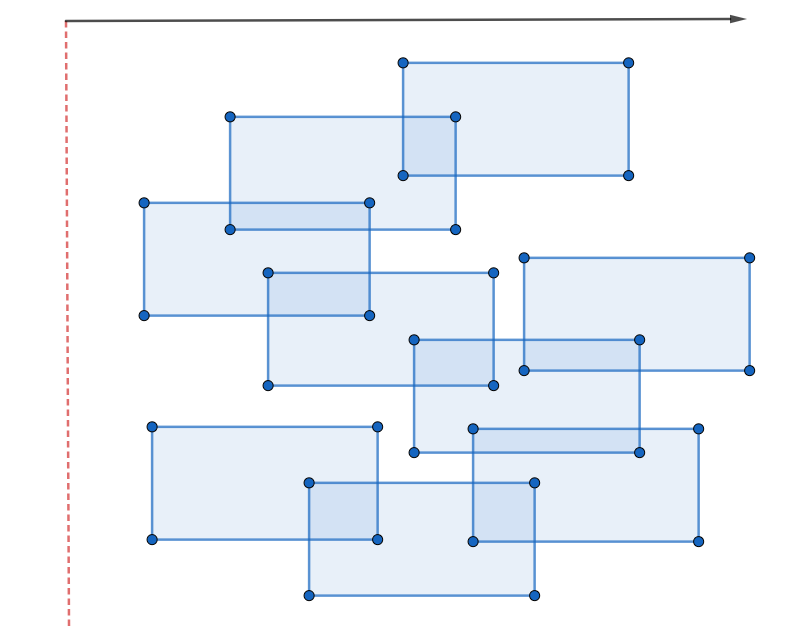
\includegraphics[scale=0.35]{images/sweepline.png}
    \end{center}
\end{frame}

\begin{frame}{掃描線的概念}
    \begin{block}{TIOJ 1224 - 矩形覆蓋面積計算}
        給你很多平面上的矩形,請求出它們覆蓋的總表面積。
    \end{block}
    \begin{center}
        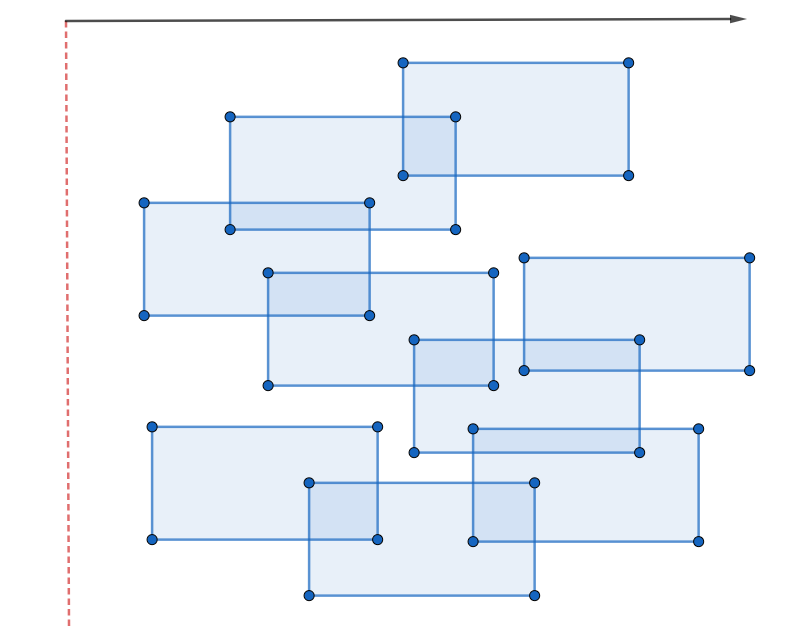
\includegraphics[scale=0.2]{images/sweepline.png}
    \end{center}
\end{frame}

\begin{frame}{掃描線的概念}
    這題是一個滿經典的掃描線搭配線段樹的題目 \\
    \vspace{2.5mm}
    我們可以使用一個鉛直的掃描線往右掃,考慮三種不同的情況 \\
    \begin{enumerate}
        \item 矩形的左邊界 (區間加值)
        \item 查詢的點 (查詢區間最小值數量)
        \item 矩形的右邊界 (區間減值)
    \end{enumerate}
    \begin{center}
        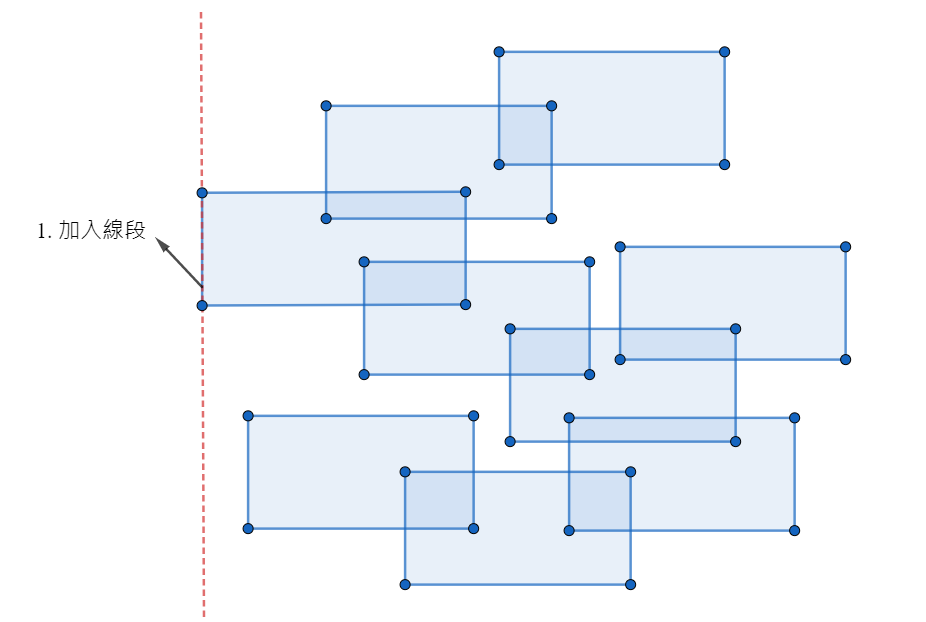
\includegraphics[scale=0.25]{images/rectangle_area_2.png}
    \end{center}
\end{frame}

\begin{frame}{掃描線的概念}
    這題是一個滿經典的掃描線搭配線段樹的題目 \\
    \vspace{2.5mm}
    我們可以使用一個鉛直的掃描線往右掃,考慮三種不同的情況 \\
    \begin{enumerate}
        \item 矩形的左邊界 (區間加值)
        \item 查詢的點 (查詢區間最小值數量)
        \item 矩形的右邊界 (區間減值)
    \end{enumerate}
    \begin{center}
        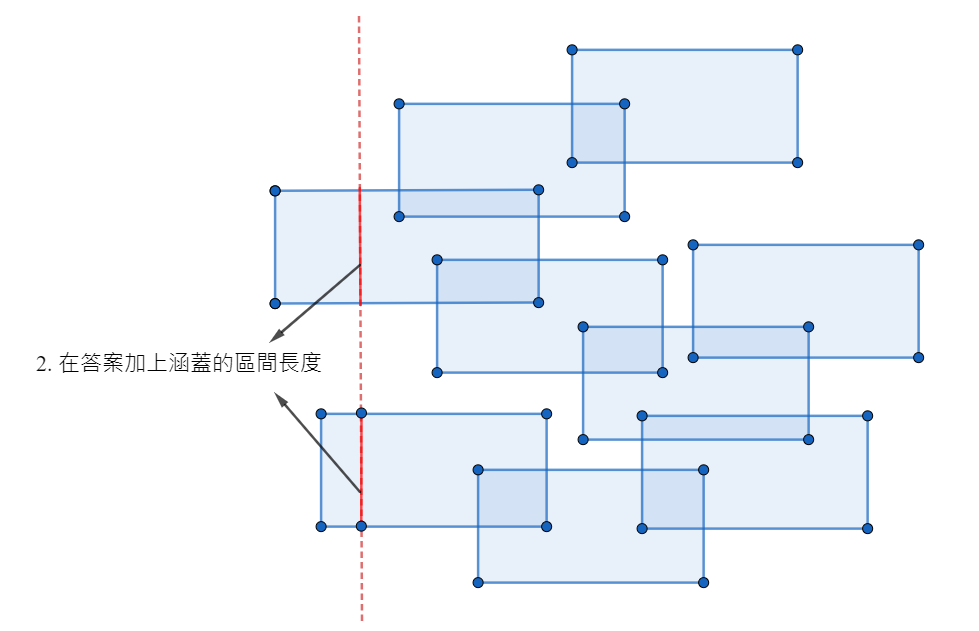
\includegraphics[scale=0.25]{images/rectangle_area_3.png}
    \end{center}
\end{frame}

\begin{frame}{掃描線的概念}
    這題是一個滿經典的掃描線搭配線段樹的題目 \\
    \vspace{2.5mm}
    我們可以使用一個鉛直的掃描線往右掃,考慮三種不同的情況 \\
    \begin{enumerate}
        \item 矩形的左邊界 (區間加值)
        \item 查詢的點 (查詢區間最小值數量)
        \item 矩形的右邊界 (區間減值)
    \end{enumerate}
    \begin{center}
        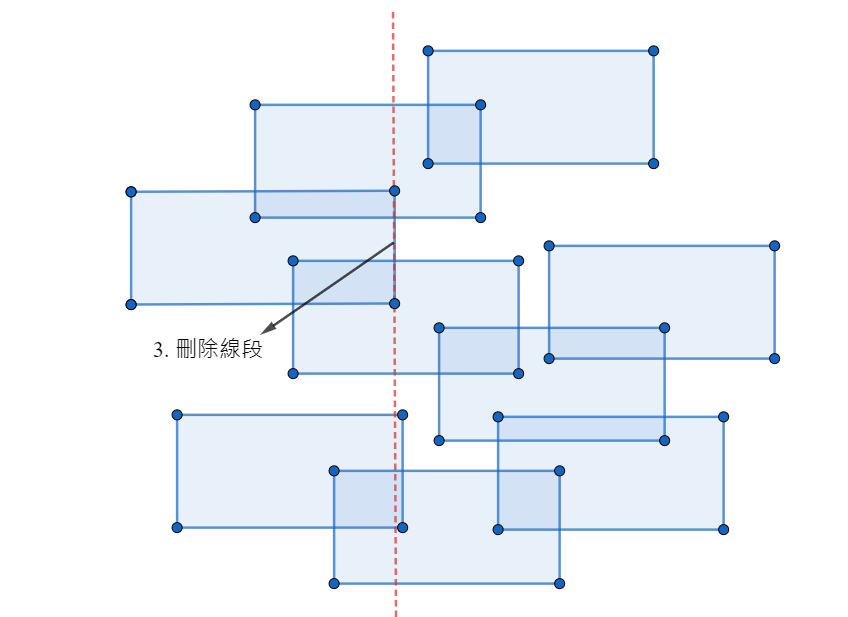
\includegraphics[scale=0.25]{images/rectangle_area_4.png}
    \end{center}
\end{frame}

\begin{frame}{掃描線的概念}
    而這三個操作,我們可以使用一棵懶標線段樹來達成。
    \begin{enumerate}
        \item 矩形的左邊界 (區間加值)
        \item 查詢的點 (查詢區間最小值數量)
        \item 矩形的右邊界 (區間減值)
    \end{enumerate}
\end{frame}

\begin{frame}{掃描線的概念}
    而這三個操作,我們可以使用一棵懶標線段樹來達成。
    \begin{enumerate}
        \item 矩形的左邊界 (區間加值)
        \item 查詢的點 (查詢區間最小值數量)
        \item 矩形的右邊界 (區間減值)
    \end{enumerate}
\end{frame}

\begin{frame}{練習題}
    \begin{block}{CSES - Intersection Points (線段交點數量)}
        給你 $n$ 個鉛直或水平的線段,問這些線段總共有多少交點。
    \end{block}
    
    \begin{block}{Codeforces 1401E - Divide Square}
        現在平面上有一個 $10^6 \times 10^6$ 的正方形以及 $n$ 個鉛直或水平的線段,問這些線段總共將這個正方形切割成了幾塊不同的區塊。
    \end{block}
\end{frame}

\section{更多例題}

\begin{frame}{一些給大家思考看看的題目}
    \begin{block}{通過最多點的直線}
        平面上有 $n$ 個點,任意畫一條直線,這條直線最多能通過幾個點?
    \end{block}
    
    \begin{block}{點到線段的最短距離}
        給你一個點 $P$ 和一個線段 $\overrightarrow{AB}$,問點 $P$ 距離線段 $\overrightarrow{AB}$ 的最短距離是多少?
    \end{block}
    
    \begin{block}{最窄寬度}
        平面上有 $n$ 個點,用兩條平行線將所有點夾住的話,兩條平行線的寬度最小可以是多窄?
    \end{block}
    
    \begin{block}{三角形數量}
        平面上有 $n$ 個點,你總共可以畫出幾個三角形
    \end{block}
\end{frame}

\end{document}